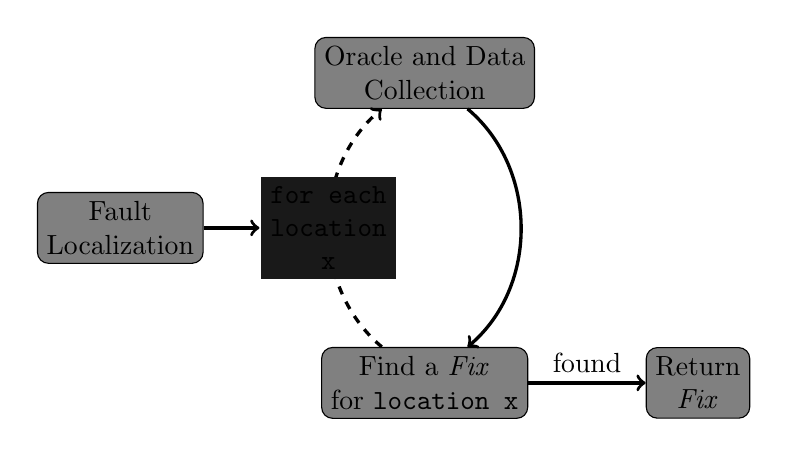
\begin{tikzpicture}[
  every matrix/.style={ampersand replacement=\&,column sep=4em,row sep=3em},
  box/.style={draw,rounded corners,fill=gray},
  flow/.style={->, very thick},
  fail/.style={->, very thick, dashed},
  every node/.style={align=center}]
  
% Position the nodes using a matrix layout
\matrix{

      \& \node[box] (test) {Oracle and Data \\ Collection};
      \& \\
      \node[box] (faultLocalization) {Fault \\ Localization};
      \& \\
      \& \node[box] (generateCandidate) {Find a \textit{Fix} \\ for \texttt{location x}};
      \& \node[box] (output) {Return \\ \textit{Fix}};
      \\
  };

% Draw the arrows between the nodes and label them.
\draw [flow] (test) to[bend left=50] (generateCandidate);
\draw [flow] (generateCandidate) to node[above] {found} (output);
\draw [fail] (generateCandidate) to[bend left=50] node[font=\ttfamily, fill=black!90] (statement) {for each \\ location \\ x} (test);
\draw [flow] (faultLocalization) -- (statement.west);

\end{tikzpicture}
